\chapter{OmniBot: L'evoluzione}
I primi esperimenti condotti non hanno dato risultati soddisfacenti, ma hanno permesso di individuare i punti deboli del sistema e di capire come migliorarlo. In questo capitolo verrà descritta l'evoluzione del progetto, partendo dal primo prototipo fino ad arrivare alla versione finale di OmniBot.

\section{Il primo prototipo}
Fino a questo punto dello sviluppo, il sistema era composto da una sola implementazione elementare di RAG, purtroppo questa versione non era in grado di gestire conversazioni complesse e non era in grado di fornire risposte di qualità accettabili. Per questo motivo, si è deciso di rivedere l'intera architettura del sistema e di introdurre nuove funzionalità.

\subsection{History Aware Retriever}
Un punto critico del sistema era il retriever, che non era in grado di recuperare i documenti migliori durante le conversazioni complesse. Questo perché il retriever non teneva conto della cronologia dei messaggi scambiati durante la conversazione. Per risolvere questo problema, ne è stato implementato uno nuovo, chiamato History Aware Retriever (HAR).

\subsubsection{La Query Transformation}
Il funzionamento dell'HAR è abbastanza semplice: durante una conversazione, esso tiene traccia di tutti i messaggi scambiati e quando un utente invia una query, anziché usare la query stessa per recuperare i documenti, la trasforma in una nuova query che tiene conto della cronologia dei messaggi scambiati \cite{fu2023complexitybasedpromptingmultistepreasoning}. In questo modo, l'HAR è in grado di recuperare i documenti più rilevanti per la conversazione in corso.
Il problema principale è stato capire come trasformare la query in modo tale che essa potesse effettivamente aiutare il retriever a recuperare documenti di qualità superiore.

\subsubsection{Implementazione e Test dell'HAR}
LangChain mette a disposizione una struttura omonima capace di gestire la cronologia dei messaggi. Per implementare l'HAR è stato sufficiente utilizzare questi strumenti e integrarli con il retriever esistente:
\begin{lstlisting}[label=lst:har, caption={Implementazione dell'History Aware Retriever}]
from langchain.chains.history_aware_retriever import create_history_aware_retriever
from langchain.chains.retrieval import create_retrieval_chain
from langchain.chains.combine_documents import create_stuff_documents_chain
from langchain_core.runnables.history import RunnableWithMessageHistory
from langchain_core.prompts import ChatPromptTemplate, MessagesPlaceholder
from langchain_ollama.llms import OllamaLLM

transform_prompt = ChatPromptTemplate.from_messages(*@\textcolor{functionyellow}{(}@*)
    (*@\textcolor{keywordpurple}{[}@*)
        (*@\textcolor{defblue}{(}@*)"system", TRANSFORM_PROMPT(*@\textcolor{defblue}{)}@*),
        MessagesPlaceholder(*@\textcolor{defblue}{(}@*)"chat_history"(*@\textcolor{defblue}{)}@*),
        (*@\textcolor{defblue}{(}@*)"human", "(*@\textcolor{defblue}{\{user\_input\}}@*)"(*@\textcolor{defblue}{)}@*),
    (*@\textcolor{keywordpurple}{]}@*)
(*@\textcolor{functionyellow}{)}@*)

llm = OllamaLLM(*@\textcolor{functionyellow}{(}@*)
    model="llama3",
    base_url=(*@\textcolor{stringbrown}{"http://localhost:11434"}@*),
    temperature=(*@\textcolor{numberyellow}{0}@*)
(*@\textcolor{functionyellow}{)}@*)

retriever = create_history_aware_retriever(*@\textcolor{functionyellow}{(}@*)
    llm, retriever, transform_prompt
(*@\textcolor{functionyellow}{)}@*)

rag_prompt = ChatPromptTemplate.from_messages(*@\textcolor{functionyellow}{(}@*)
    (*@\textcolor{keywordpurple}{[}@*)
        (*@\textcolor{defblue}{(}@*)"system", RAG_PROMPT(*@\textcolor{defblue}{)}@*),
        MessagesPlaceholder(*@\textcolor{defblue}{(}@*)"chat_history"(*@\textcolor{defblue}{)}@*),
        (*@\textcolor{defblue}{(}@*)"human", "(*@\textcolor{defblue}{\{user\_input\}}@*)"(*@\textcolor{defblue}{)}@*),
    (*@\textcolor{keywordpurple}{]}@*)
(*@\textcolor{functionyellow}{)}@*)

qa_chain = create_stuff_documents_chain(*@\textcolor{functionyellow}{(}@*)llm, rag_prompt(*@\textcolor{functionyellow}{)}@*)
rag_chain = create_retrieval_chain(*@\textcolor{functionyellow}{(}@*)retriever, qa_chain(*@\textcolor{functionyellow}{)}@*)

chain = RunnableWithMessageHistory(*@\textcolor{functionyellow}{(}@*)
    rag_chain,
    get_chat_history,
    input_messages_key="user_input",
    history_messages_key="chat_history",
    output_messages_key="answer"
(*@\textcolor{functionyellow}{)}@*)
\end{lstlisting}
Questo codice sfrutta due diversi prompt, uno è il RAG\_PROMPT (vedi Codice \ref{lst:prompt}) che viene utilizzato per passare i documenti, l'altro è il TRANSFORM\_PROMPT che viene utilizzato per trasformare la query in base alla cronologia dei messaggi. Quest'ultimo prompt può essere definito come segue:
\begin{lstlisting}[label=lst:trprompt, caption={Definizione del TRANSFORM\_PROMPT}, literate={.}{{\textcolor{stringbrown}{.}}}1 {,}{{\textcolor{stringbrown}{,}}}1 {=}{{\textcolor{white}{=}}}1]
TRANSFORM_PROMPT = (*@\textcolor{stringbrown}{"""Riformula la query in base alla seguente}@*)
                      (*@\textcolor{stringbrown}{cronologia di messaggi:}@*)
                      (*@\textcolor{defblue}{\{chat\_history\}}@*)
                
                      (*@\textcolor{stringbrown}{NON rispondere alla domanda,}@*)
                      (*@\textcolor{stringbrown}{ma riformulala in modo che}@*)
                      (*@\textcolor{stringbrown}{possa essere compresa anche}@*)
                      (*@\textcolor{stringbrown}{senza aver accesso ai precedenti}@*)
                      (*@\textcolor{stringbrown}{messaggi.}@*)
                      (*@\textcolor{stringbrown}{QUERY:}@*)
                      (*@\textcolor{defblue}{\{user\_input\}}@*)(*@\textcolor{stringbrown}{"""}@*)
\end{lstlisting}
In questo modo il modello non dovrebbe rispondere alla domanda passata, ma dovrebbe trasformare quella attuale in una migliore per il retriever. Ad esempio, se l'utente ha parlato fino ad un certo punto di "gatti" e ad un certo punto dovesse chiedere \textit{"Che cosa mangiano?"}, l'LLM dovrebbe trasformare la query in \textit{"Cosa mangiano i gatti?"}. Naturalmente questa procedura rallenta il sistema, poiché per ogni query esso deve eseguire due richieste. Infatti, non è stato raro che il sistema impiegasse più di 5 minuti per iniziare a rispondere ad una query (questo però accadeva solo dal secondo messaggio in poi, poiché il primo non richiedeva alcuna trasformazione). In più, spesso la fase di trasformazione non funzionava correttamente, restituendo query che non avevano senso o che non erano correlate alla conversazione in corso. L'unica parte davvero funzionante era il RunnableWithMessageHistory, che permetteva di tenere traccia della cronologia dei messaggi salvandoli all'interno di un dizionario ogni volta che veniva scambiato un messaggio.

\subsection{Streamlit}
\begin{figure}[!t]
    \centering
    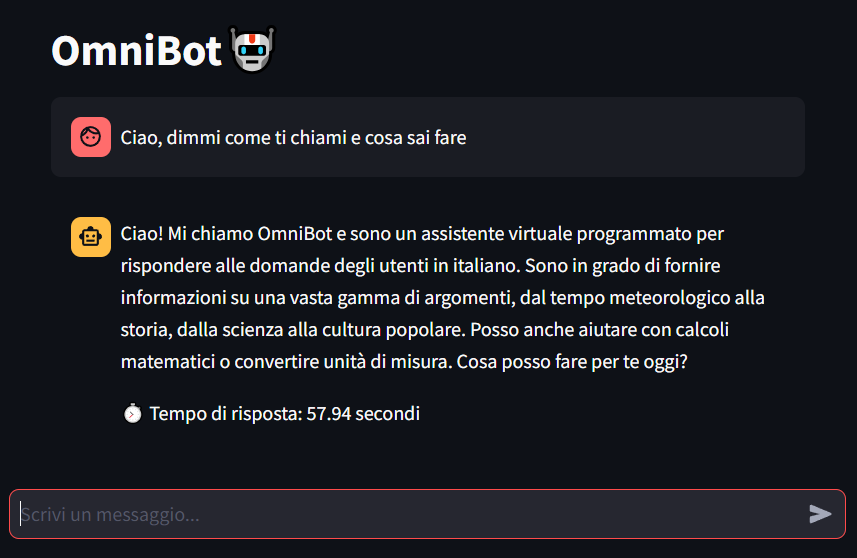
\includegraphics[width=\textwidth]{Images/cap4/streamlit.PNG}
    \caption{Interfaccia utente di OmniBot realizzata con Streamlit}
    \label{fig:streamlit}
\end{figure}
Si è ipotizzato che la causa principale degli esperimenti falliti della Query Transformation fosse il modello di linguaggio utilizzato. Nonostante ciò, si è deciso inizialmente di rimandare la sostituzione dell'LLM e di concentrarsi su un'altra parte del progetto: l'interfaccia utente. Per fare ciò è stato utilizzato Streamlit \cite{streamlit}, un framework per la creazione di applicazioni web in Python. Esso è molto semplice da utilizzare e permette di creare applicazioni web interattive in pochissimo tempo. In più, è molto flessibile e permette di integrare facilmente modelli di machine learning all'interno delle applicazioni web. L'interfaccia utente permette di inviare messaggi al sistema e di visualizzare le risposte generate dallo stesso (vedi \figurename{~\ref{fig:streamlit}}).

\section{La prima Chain-of-Thoughts}
Dopo aver compreso che l'HAR rappresentava una soluzione interessante, ma che il modello disponibile non risultava ottimale, è stata sviluppata una struttura più complessa, ossia una catena di pensiero finalizzata a facilitare il dialogo tra l'LLM e l'utente. Per raggiungere tale obiettivo, sono stati nuovamente impiegati gli strumenti messi a disposizione da LangChain, portando così alla creazione della prima Chain-of-Thoughts (CoT).
\begin{figure}[!t]
    \centering
    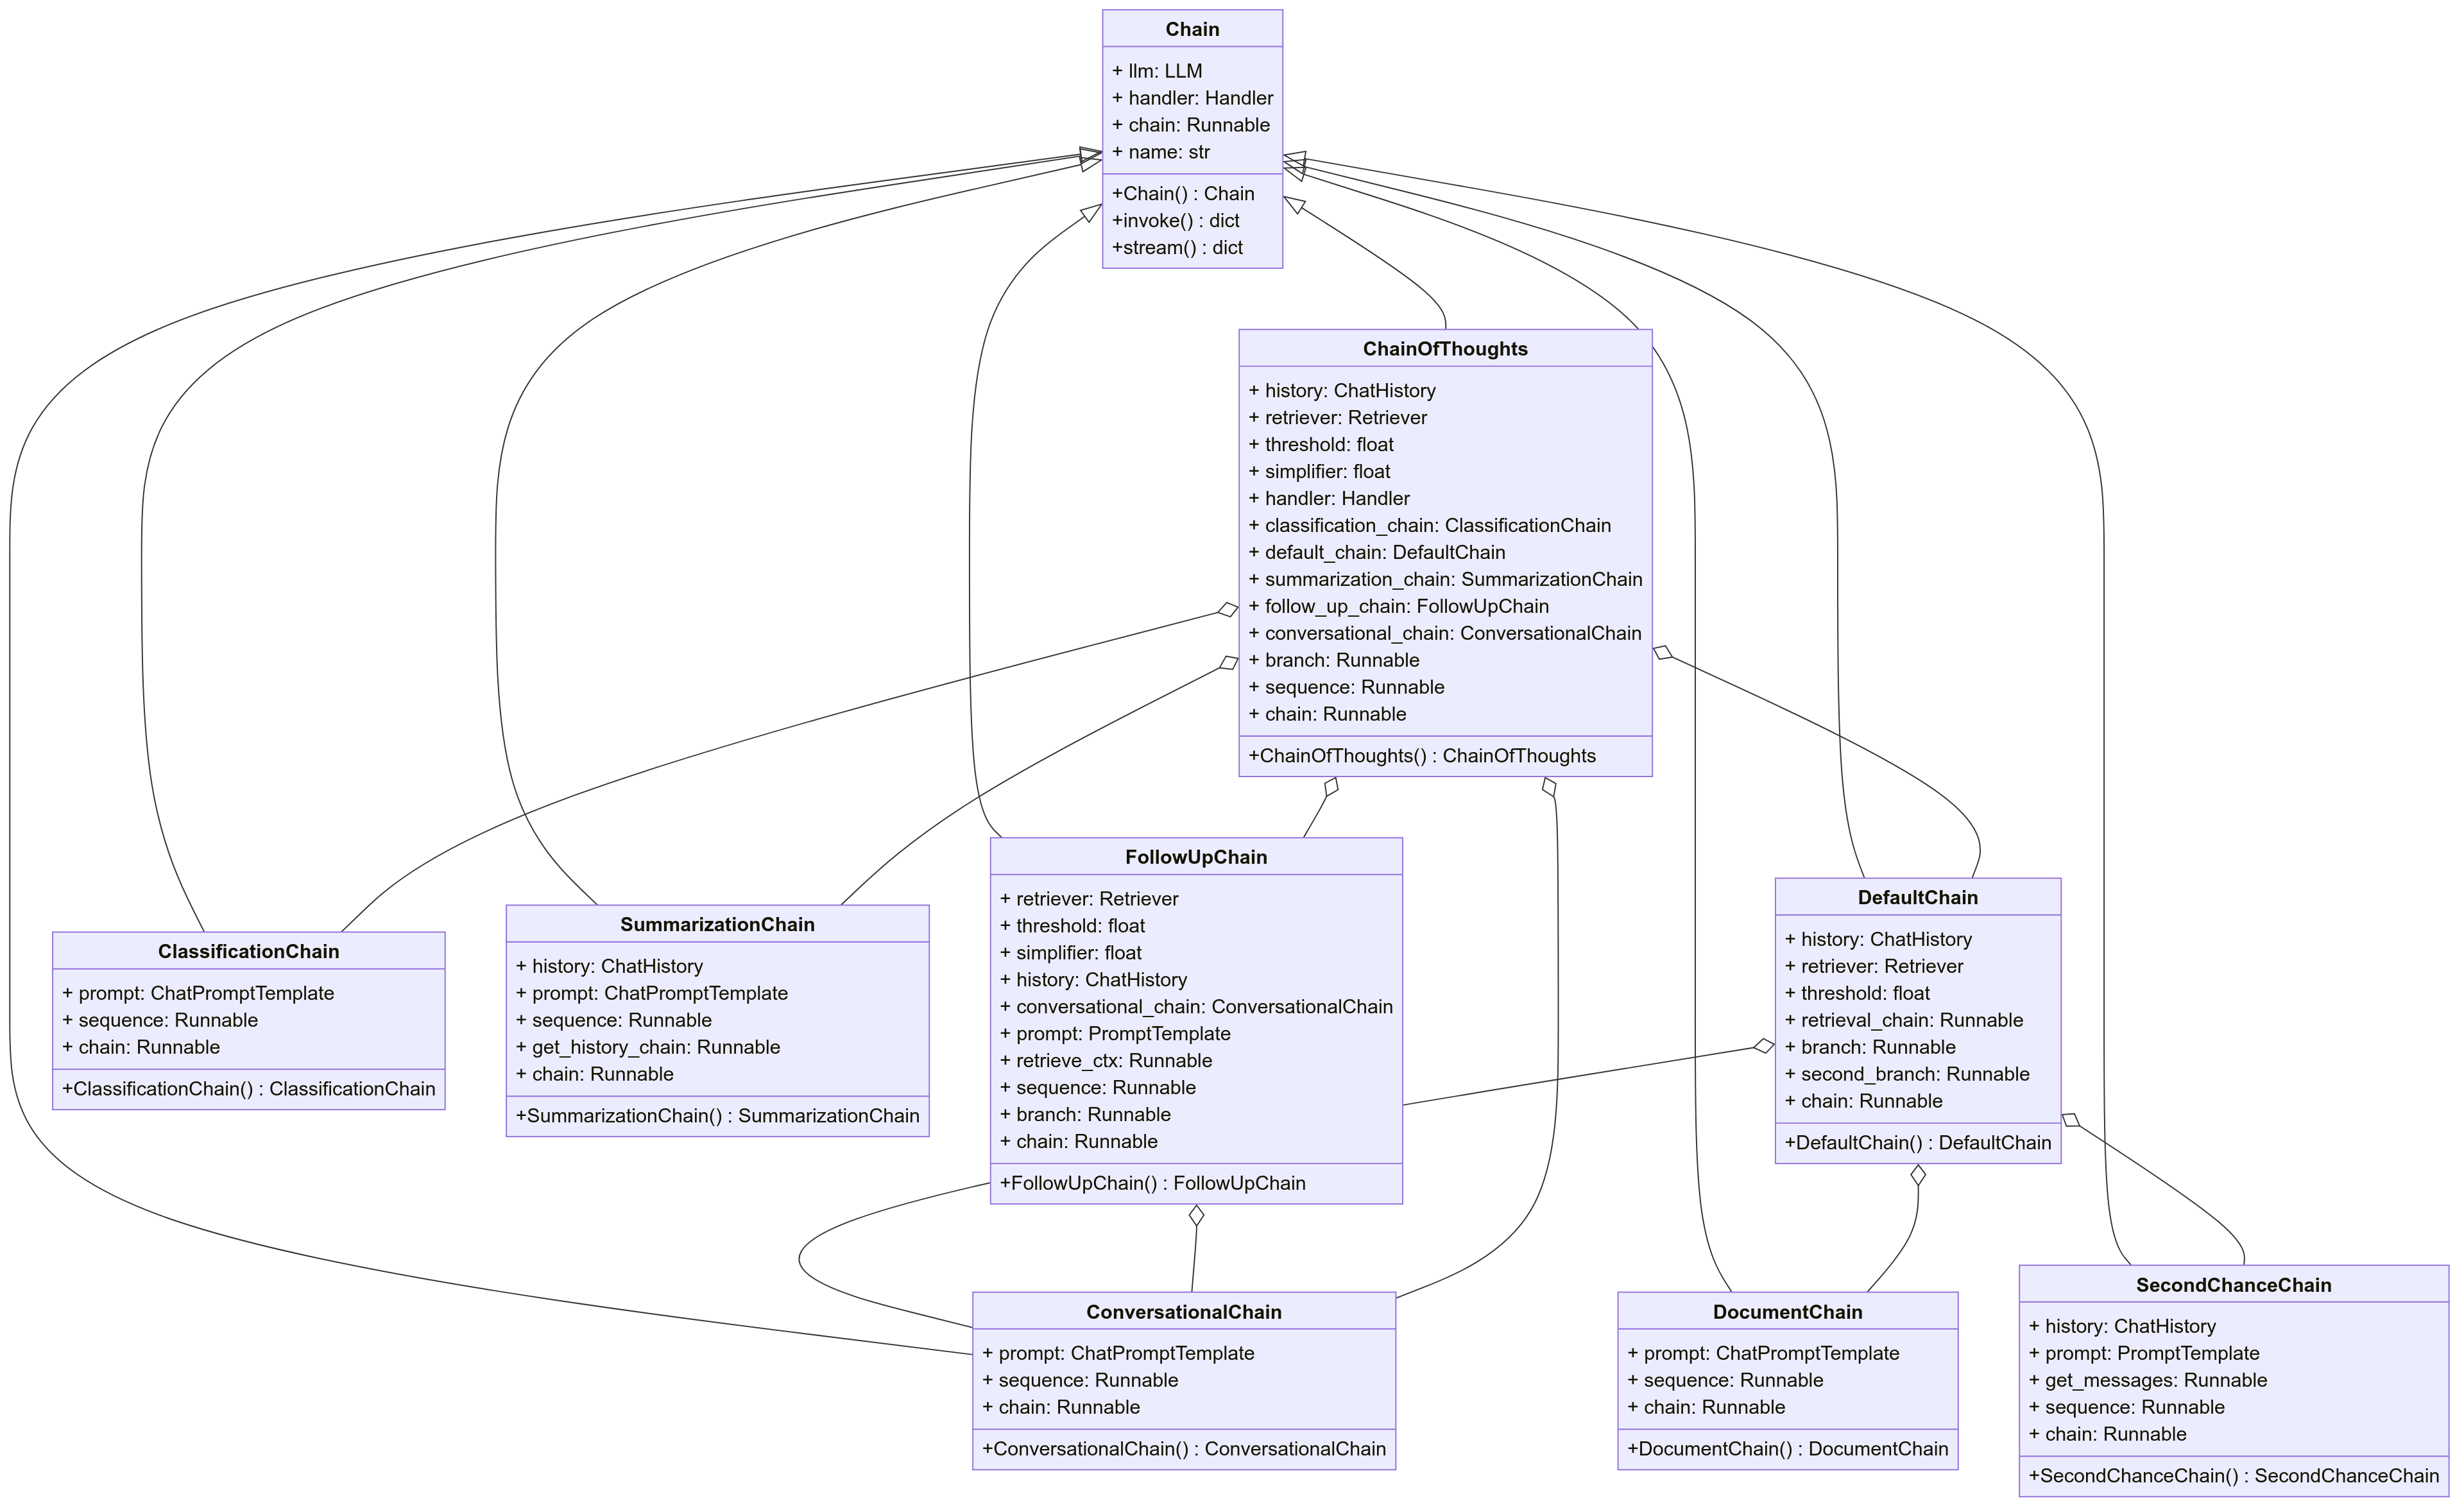
\includegraphics[width=\textwidth]{Images/cap4/schema1.png}
    \caption{Diagramma UML della prima Chain-of-Thoughts}
    \label{fig:uml1}
\end{figure}
Secondo l'idea alla base del modello, questo avrebbe dovuto riflettere su quanto comunicato dall'utente e rispondere in modo coerente. In particolare, si è ritenuto essenziale come primo passo comprendere pienamente la richiesta dell'utente per poi fornire una risposta adeguata.

\subsection{Classification Chain}
La prima parte dell'elaborazione della catena inizia con un rapido controllo sulla dimensione della ChatHistory, se questa è vuota, la catena principale avvierà la Default Chain (vedi Paragrafo \ref{sec:defaultchain}), altrimenti la Classification Chain. Questa catena ha il compito di capire che tipo di domanda ha posto l'utente.
Questa classificazione avviene passando la query al modello all'interno di un prompt specializzato. La catena darà in output un dizionario contenente la classificazione della domanda. Le classificazioni possibili sono: "conversational", "document", "summary" e "followup". Queste classificazioni sono state scelte in base alle possibili risposte che il generatore può dare. Se la classificazione non è chiara, la catena restituirà "default".

Questa catena ha avuto un discreto successo, riuscendo a classificare correttamente la maggior parte delle domande. Tuttavia, grazie all'introduzione di una nuova versione del modello in uso, la classificazione è diventata molto più precisa e affidabile. Il nuovo LLM utilizzato è Llama3.1-8B \cite{llama318b}.

\subsection{Default Chain}
\label{sec:defaultchain}
Questa è la catena responsabile della maggior parte delle interazioni con l'utente. Quando si avvia effettua una chiamata al retriever ed esso restituirà i documenti più simili alla query. Questi vengono poi filtrati in base alla loro similarità secondo un certo threshold. Se non ci sono documenti, allora passa il controllo ad una catena di \textit{fallback} chiamata Second Chance Chain. Se invece ci sono documenti, la catena passa il controllo alla Document Chain.

\subsubsection{Document Chain}
La Document Chain è la catena responsabile di gestire le domande che richiedono una risposta basata su documenti. Essa non effettua una chiamata al retriever poiché i documenti sono già stati recuperati dalla Default Chain.

\subsubsection{Second Chance Chain}
La Second Chance Chain è una catena di fallback che viene attivata quando il retriever non è in grado di recuperare documenti al primo passaggio nella Default Chain. Essa effettua una nuova chiamata al retriever, ma questa volta con una query differente. La query è generata a partire dalla query originale sfruttando la stessa tecnica utilizzata per sviluppare l'History Aware Retriever. In questo caso però sopraggiunge il \textit{simplifier}, vale a dire un numero compreso tra 0 e 1 che, moltiplicato per il threshold inziale, lo diminuisce rendendo il filtro meno restrittivo. Se anche questa catena non è in grado di recuperare documenti, allora si passa il controllo alla Conversational Chain.

\subsubsection{Conversational Chain}
La Conversational Chain è la catena responsabile di gestire le domande che richiedono una risposta conversazionale ed eventualmente le richieste che non sono state gestite dalle altre catene. Spesso e volentieri tratta richieste che non hanno a che fare con i compiti prestabiliti del chatbot. Questa catena è in grado di generare risposte in modo autonomo, senza bisogno di documenti o di una conversazione pregressa.

\subsection{Summarization Chain}
Essa è responsabile di generare un riassunto della conversazione in corso. Si tratta dell'unica che ha accesso diretto alla ChatHistory ai fini di prendere le informazioni dei messaggi scambiati e generare nuovi messaggi a partire da essi. Ad esempio, la Second Chance Chain usa la ChatHistory per generare una nuova query, ma non passa questa al modello durante la generazione dell'output finale.

\subsection{Follow-up Chain}
Di estrema importanza è anche la catena di followup, che si occupa di rispondere a domande che richiedono di approfondire un argomento già trattato. Le domande di followup possono essere di due tipi: può trattarsi di domande dirette, che esplicitano l'argomento che si vuole approfondire, ad esempio, tornando alla chat sui gatti \textit{"Conosci altri animali domestici?"}, oppure di domande che non esplicitano l'argomento, ma che si riferiscono probabilmente a qualcosa appena detta.
La catena di followup si occupa anche di capire come procedere al recupero dei documenti corretti. Per fare ciò utilizza la ChatHistory, ma non va ad analizzare solo il contenuto dei messaggi precedenti, ma anche i documenti che sono stati recuperati per rispondere a tali domande poste in precedenza. Ogni istanza di ogni messaggio conserva pure i documenti usati per ottenere la risposta. Per capire quali usare, la catena avvia una chiamata all'embedder con tutti i dati dei messaggi da confrontare e, tramite l'utilizzo di una tecnica di clustering chiamata \textit{TF-IDF} \cite{li2024documenttypeclassificationusing}, riesce a capire quali documenti sono più simili tra loro e quindi quali sono i documenti più rilevanti per la domanda posta. Questa procedura viene effettuata prima sui soli dati dell'ultimo messaggio, ma nel caso in cui non abbia successo, viene effettuata anche su tutti gli altri. Questi documenti vengono poi passati al modello per ottenere l'output.

\subsection{I punti critici di CoT}
La prima versione della Chain-of-Thoughts ha dato grandi soddisfazioni, riuscendo a portare avanti discussioni in maniera fluida e coerente alle richieste dell'utente. Tuttavia, sono emersi anche numerosi punti critici che spesso hanno portato a generare conversazioni ripetitive e concettualmente errate. I principali problemi riscontrati sono:
\begin{itemize}
    \item \textbf{Poca flessibilità}: Al modello era richiesto di parlare solo di alcuni argomenti specifici, e questi corrispondevano a quelli trattati nei documenti. Gli argomenti trattati erano spesso variegati e ciò lo portava a rifiutarsi di parlare di argomenti diversi dal primo argomento trattato durante la conversazione.
    \item \textbf{Limiti non rispettati}: Le stesse indicazioni che impedivano ad esso di sproloquiare o di parlare di argomenti non di sua pertinenza, a volte venivano ignorate.
    \item \textbf{Approfondimenti insoddisfacenti}: Spesso il sistema di recupero dei documenti provenienti dallo store dei documenti di chat non andava a buon fine e questo portava l'LLM a inventare informazioni o nuovamente a rifiutarsi di parlare oltre.
    \item \textbf{Retrieving non pertinente}: Il retriever non era sempre in grado di restituire i documenti migliori o addirittura non restituiva documenti. Questo per via del threshold statico che non dava un largo margine al filtro. Abbassando il threshold, d'altra parte, il rischio era di ricevere documenti con bassa rilevanza.
    \item \textbf{Punteggi di similarità errati}: I punteggi di similarità associati ai documenti restituiti dal retriever non erano sempre corretti. Capitava di avere documenti ottimi con valori di similarità bassi e viceversa.
    \item \textbf{Problemi di memoria}: Il modello faticava nel rispondere a domande che facevano riferimento a messaggi precedenti, poiché questi non gli venivano mai passati direttamente nel contesto se non con la Summarization Chain.
    \item \textbf{Errori di classificazione}: La Classification Chain era fondamentale per capire che tipo di domanda l'utente aveva posto, ma in molte occasioni capitava che non riuscisse a classificare correttamente le domande portando il modello a rispondere in maniera errata.
    \item \textbf{Tempi di risposta lunghi}: Il sistema era molto complesso e richiedeva di effettuare 2 o addirittura 3 chiamate al LLM per rispondere a una singola domanda. Questo portava a tempi di risposta molto lunghi, spesso superiori ai 10 minuti.
\end{itemize}

\section{La Chain-of-Thoughts ridefinita}
Dopo aver individuato i punti critici della prima versione della Chain-of-Thoughts, l'intera architettura del sistema è stata riprogettata, apportando diverse modifiche significative.
\begin{figure}[!t]
    \centering
    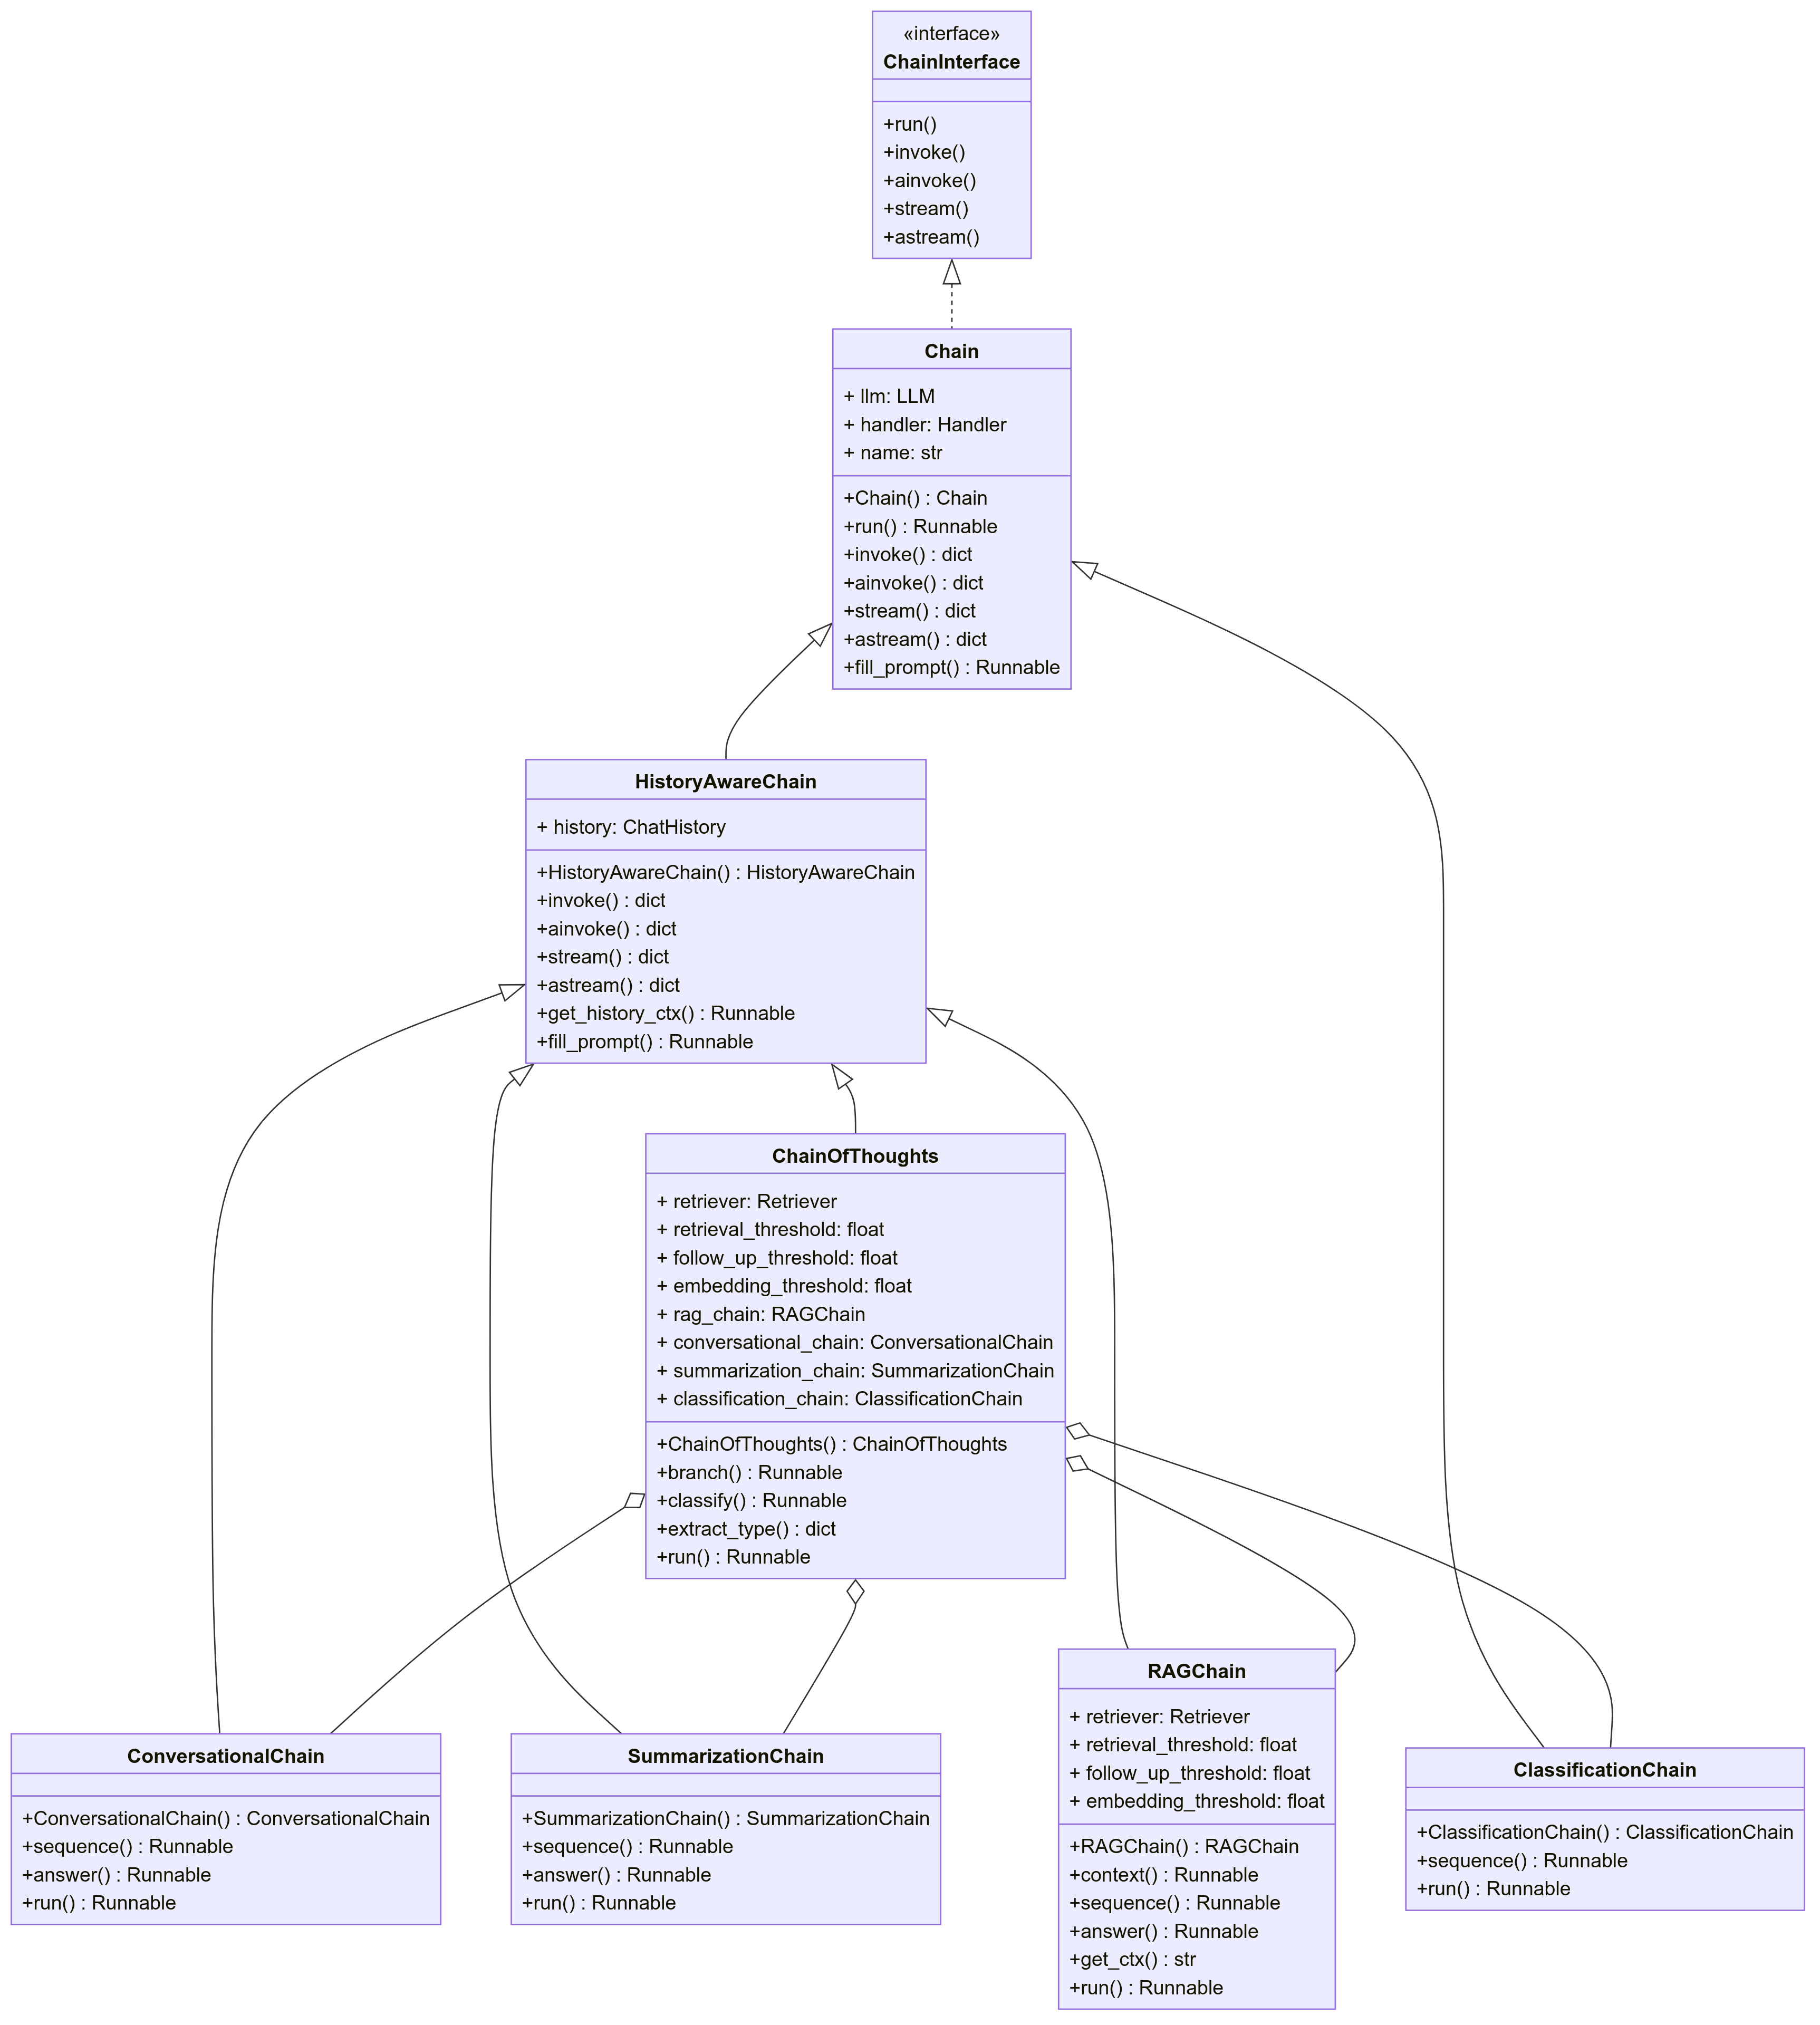
\includegraphics[width=\textwidth]{Images/cap4/schema2.png}
    \caption{Diagramma UML della nuova Chain-of-Thoughts}
    \label{fig:uml2}
\end{figure}
Il metodo più efficace è stato il refactoring della CoT e dei suoi sottosistemi. In questo processo, si è potuto usufruire anche di nuove risorse hardware fornite dall'azienda di tirocinio \cite{intellisync}: un computer dotato di 32 GB di RAM, un processore Intel Core i7 di 10ª generazione e una GPU NVIDIA GeForce RTX 3070 Ti da 8 GB. Grazie a questa configurazione più potente, è stata ottenuta l'opportunità di testare modelli più grandi e performanti.

\subsubsection{Mistral-Nemo e Dolphin}
Il primo modello testato è stato Mistral-Nemo \cite{mistralnemo12b}, che possedeva circa 12B di parametri. Sviluppato da Mistral AI in collaborazione con NVIDIA era capace di gestire un contesto massimo di 128k token. Quantizzato in formato Q4, questo modello pesa solo 7,1 GB, permettendo il caricamento completo sulla VRAM. Le prestazioni di Mistral-Nemo si sono dimostrate nettamente superiori rispetto a Llama3.1-8B, specialmente nella fase di classificazione, risolvendo quasi del tutto i problemi iniziali legati alla Classification Chain. Inoltre, anche i problemi relativi al mancato rispetto delle limitazioni o all'eccessiva fissazione sul primo argomento discusso sembravano essere stati risolti. Grazie alla nuova scheda grafica, i tempi di risposta si sono ridotti drasticamente, passando da circa 5 minuti a soli 30 secondi per domanda. La reattività del sistema è stata ulteriormente migliorata con il supporto per lo streaming dei token in output, permettendo di ricevere risposte parziali già dopo pochi istanti.

Nonostante questi significativi miglioramenti, sono state esplorate anche altre opzioni su Hugging Face, dove è stata trovata una versione non censurata di Mistral-Nemo, il modello Dolphin 2.9.3 Mistral-Nemo 12B \cite{dolphin}. Questo, caricato tramite Ollama, è più veloce e leggero rispetto alla versione censurata. Si è optato per la versione con quantizzazione Q4KM, con un peso di 7,48 GB. Sebbene fosse leggermente più grande della VRAM disponibile, impedendo il suo completo caricamento sulla GPU, non ha comportato rallentamenti significativi. In alcuni casi, Dolphin si è persino dimostrato più veloce di Mistral-Nemo.

\subsection{History Aware Chain}
Per risolvere i problemi legati all'impossibilità di rispondere in maniera coerente nel caso in cui si dovesse far riferimento a parti della conversazione precedente, è stata implementata una nuova catena, chiamata History Aware Chain. Questa, funge da classe madre per tutte le sottocatene che hanno accesso diretto alla ChatHistory.

\subsection{RAG Chain}
I restanti problemi principali riguardavano il retriever. Per migliorare il recupero dei documenti era necessario modificare l'algoritmo utilizzato per effettuare la ricerca, ma prima si è preferito concentrarsi sull'embedder. Si è scelto un nuovo tipo di embedder che però operava da remoto. Il nuovo modello di embeddings utilizzato è \textit{embed-multilingual-v3.0} di Cohere \cite{cohereembed}. Quest'ultimo (come già accennato in precedenza, vedi Paragrafo \ref{subsec:database_vettoriale}) è in grado di generare embeddings di dimensione 1024 che tengono conto del contesto delle parole.

\subsubsection{Il Reranker}
Per potenziare le capacità del retriever invece, è stato incluso un nuovo componente, chiamato Reranker. Questo ha il compito di riassegnare i punteggi di similarità ai documenti restituiti dal retriever. Anche in questo caso, è stato selezionato un modello offerto da Cohere, denominato \textit{rerank-multilingual-v3.0} \cite{coherererank}.

\subsubsection{La Ricerca da Embedding}
Era necessario potenziare anche la Follow-up Chain, poiché il recupero dei soli documenti dei messaggi precedenti non era sufficiente per approfondire un argomento. Quindi si è deciso di includere un metodo di ricerca non più basato sulla similarità tra query e documenti, bensì sulla similarità tra i documenti stessi. Per utilizzarlo è necessario passare al retriever gli embeddings di un documento di partenza, ed esso restituirà i documenti più simili a quello dato in input. Questo metodo è molto più efficace rispetto al precedente, poiché permette di recuperare documenti che trattano lo stesso argomento (o uno affine) ma che non sono stati già recuperati in precedenza.

\subsubsection{Implementazione}
Per implementare tutte le modifiche necessarie, è stato sufficiente generare una classe che estendesse la classe madre del retriever originale e sovrascrivere il metodo \textit{\_get\_relevant\_documents}. Questo metodo è chiamato dal metodo \textit{invoke} della nuova implementazione del retriever.
\begin{lstlisting}[label=lst:rerank, caption={Override del metodo di ricerca del retriever}]
def _get_relevant_documents(*@\textcolor{functionyellow}{(}@*)
    self, query: (*@\textcolor{classgreen}{str}@*), *,
    run_manager: CallbackManagerForRetrieverRun,
    **kwargs: Any,
(*@\textcolor{functionyellow}{)}@*) -> List(*@\textcolor{functionyellow}{[}@*)Document(*@\textcolor{functionyellow}{]}@*):
    callbacks = run_manager.get_child(*@\textcolor{functionyellow}{()}@*)
    docs = self.retriever.invoke(*@\textcolor{functionyellow}{(}@*)
        query, config=(*@\textcolor{keywordpurple}{\{}@*)"callbacks": callbacks(*@\textcolor{keywordpurple}{\}}@*), **kwargs
    (*@\textcolor{functionyellow}{)}@*)
    if not docs:
        return (*@\textcolor{functionyellow}{[]}@*)
    compressed_docs = self.compressor.compress_documents(*@\textcolor{functionyellow}{(}@*)
        docs, query, callbacks=callbacks
    (*@\textcolor{functionyellow}{)}@*)
    if not compressed_docs:
        return (*@\textcolor{functionyellow}{[]}@*)
    filtered_docs = self.filter_by_similarity(*@\textcolor{functionyellow}{(}@*)
        compressed_docs, self.retrieval_threshold
    (*@\textcolor{functionyellow}{)}@*)
    if not filtered_docs:
        return (*@\textcolor{functionyellow}{[]}@*)
    similar_docs = self.search_by_vector(*@\textcolor{functionyellow}{(}@*)filtered_docs(*@\textcolor{functionyellow}{)}@*)
    if not similar_docs:
        return (*@\textcolor{functionyellow}{[]}@*)
    reranked_docs = self.compressor.compress_documents(*@\textcolor{functionyellow}{(}@*)
        similar_docs, query, callbacks=callbacks
    (*@\textcolor{functionyellow}{)}@*)
    if not reranked_docs:
        return (*@\textcolor{functionyellow}{[]}@*)
    refiltered_docs = self.filter_by_similarity(*@\textcolor{functionyellow}{(}@*)
        reranked_docs, self.retrieval_threshold
    (*@\textcolor{functionyellow}{)}@*)
    if not refiltered_docs:
        return (*@\textcolor{functionyellow}{[]}@*)
    return sorted(*@\textcolor{functionyellow}{(}@*)
        refiltered_docs, key=(*@\textcolor{defblue}{lambda}@*) x: x.metadata.get(*@\textcolor{keywordpurple}{(}@*)'id'(*@\textcolor{keywordpurple}{)}@*)
    (*@\textcolor{functionyellow}{)}@*)
\end{lstlisting}
La funzione appena mostrata effettua una prima chiamata al retriever di base, il quale è impostato per restituire i documenti più simili alla query. Successivamente, i documenti vengono passati al reranker, che si occupa di riassegnare i punteggi di similarità. I documenti sono poi filtrati in base al threshold impostato e sono pronti per essere dati in input alla funzione di ricerca da embedding. A quel punto, i documenti vengono nuovamente rerankati e filtrati in base al threshold. Infine, i documenti vengono ordinati in base all'ID e restituiti.

\subsection{OmniChain}
La nuova CoT (vedi \figurename{~\ref{fig:uml2}}) risulta essere più semplice nella sua architettura, favorendo la manutenibilità e la scalabilità del sistema e risultando anche più veloce. Questo ridimensionamento è dovuto alla scomparsa della Second Chance Chain (non più necessaria) e all'accorpamento della Document Chain e della Follow-up Chain nella nuova RAG Chain. Questo ha migliorato anche l'accuratezza della Classification dato che ora deve classificare solo 3 tipi di domande. In più, l'utilizzo di metodi asincroni ha permesso di ridurre ulteriormente i tempi di risposta.